\documentclass[10pt,twocolumn,letterpaper]{article}
 \pdfoutput=1
\usepackage{cvpr}
\usepackage{times}
\usepackage{epsfig}
\usepackage{graphicx}
\usepackage{amsmath}
\usepackage{amssymb}
\usepackage{bm}
\usepackage{subcaption}
%\usepackage{slashbox}
\usepackage{color}
\usepackage[english]{babel}
%\usepackage[linesnumbered,ruled,vlined]{algorithm2e}
\usepackage[breaklinks=true,bookmarks=false]{hyperref}
\usepackage{booktabs}
%\usepackage{caption}
\usepackage{algorithm}
\usepackage{algorithmic}

\DeclareCaptionLabelFormat{noname}{#2}
\captionsetup[algorithm]{labelformat=noname}

\newlength\myindent
\setlength\myindent{2em}
\newcommand\bindent[1][\myindent]{%
  \begingroup
  \setlength{\itemindent}{#1}
  \addtolength{\algorithmicindent}{#1}
}
\newcommand\eindent{\endgroup}


\usepackage{multirow}
\newcommand{\ra}[1]{\renewcommand{\arraystretch}{#1}}

\newcommand{\argmin}{\operatornamewithlimits{argmin}}
\cvprfinalcopy

\def\cvprPaperID{16} % *** Enter the CVPR Paper ID here
\def\httilde{\mbox{\tt\raisebox{-.5ex}{\symbol{126}}}}
\begin{document}

\title{DeepAutoTrack (DAT): Vehicle Trajectory Prediction for Autonomous Driving}

\author{Di Wu, Zhennan Wang, Yi Tang,  Wenbin Zou, Xia Li\\
Shenzhen University\thanks{Shenzhen Key Lab of Advanced Telecommunication and Information Processing, College of Information Engineering, Shenzhen University.}\\
{\tt\small dwu,...@szu.edu.cn}}
\maketitle
%%%%%%%%% ABSTRACT
\begin{abstract}
% State the problem, your approach and solution, and the main contributions of the paper. Include little if any background and motivation. Be factual but comprehensive. The material in the abstract should not be repeated later word for word in the paper.

Vision-based deep neural networks are crucial components for autonomous driving in terms of visual understanding and decision making.
These models need to be temporally consistent and visually interpretable.
Most recent works focus on using static images for understanding visual semantics, ignoring the temporal consistency of driving conditions; or adopt end-to-end architectures for learning the pilot networks, providing limited interpretability.
In this paper, we raise the question of ``can we predict car's future odometry given previous egomotion visual input?".
The proposed system stems from the issue of human driver reaction time in the autonomous driving context.
Our dual-staged model firstly applies modern convolutional object detectors for spotting traffic participants (i.e., cars in this paper) and robustly tracks the targets of interest.
Then, a novel SEG-LSTM network is incorporated to fuse the multiple-streams from past frames and then predict targets' future trajectories.
We demonstrate the feasibility of predicting future trajectories of vehicles for assisting mediated perception.
 We also show the effectiveness of using privileged information (e.g., scene semantics) further boost the prediction accuracy across diverse traffic conditions.
\end{abstract}
%%%%%%%%% BODY TEXT
%%% Andrje Karpathy's blog: http://karpathy.github.io/2016/09/07/phd/
%%% Another great resource on this topic is Tips for Writing Technical Papers from Jennifer Widom.
%%% https://cs.stanford.edu/people/widom/paper-writing.html
\section{Introduction}

%\textbf{\emph{1.1 What is the problem?}}

Currently, there are two major paradigms for autonomous driving systems built upon vision-based input~\cite{chen2015deepdriving}: mediated perception approaches that firstly explain the vision input and then parse the scene to make a driving policy (usually by a controller with if-then-else rules); and behaviour reflex approaches that directly map the vision input to a driving policy by a regressor.
In this paper, in the framework of first paradigm, we try to tackle the problem of predicting future trajectories of vehicles given its past information.

%\textbf{\emph{1.2. Why is it interesting and important?}}

 Being able to predict other traffic participants' future trajectories is important because it can help to prevent self-driving car from running into other cars. We need to know not just where other cars are, as in the localization case, but also how fast they are moving in order to avoid collisions.
For a human driver, reaction time is a crucial factor that includes recognizing the light has changed, deciding to continue or brake, and if stopping engaging the brake (remove foot from accelerator and apply brake). Accident reconstruction specialists commonly use 1.5 seconds~\cite{mcgehee2000driver}.
Therefore, the ability to predict traffic participants' \emph{future} trajectories will greatly benefits the mediated perception approach's driving policy decision making.


%\textbf{\emph{1.3. Why is it hard? (Or why do naive approaches fail?)}}

Nonetheless, vehicles trajectory prediction is a challenging problem: by dissecting visual scene understanding individually (\emph{e.g.,} object detection, semantic segmentation, instance segmentation),  there are still many open challenges for computer vision community.
In addition, scene parsing results contain quite some spurious information.
Existing methods for scene parsing also mainly focus on static images.
However, autonomous driving is intrinsically a dynamic problem. Human driver makes decision by sequence of input frames instead of simply one static frame.
Therefore, temporal consistency among continuous frames should also be taken into consideration when designing the interpretable system.


\begin{figure}[t]
        \centering
        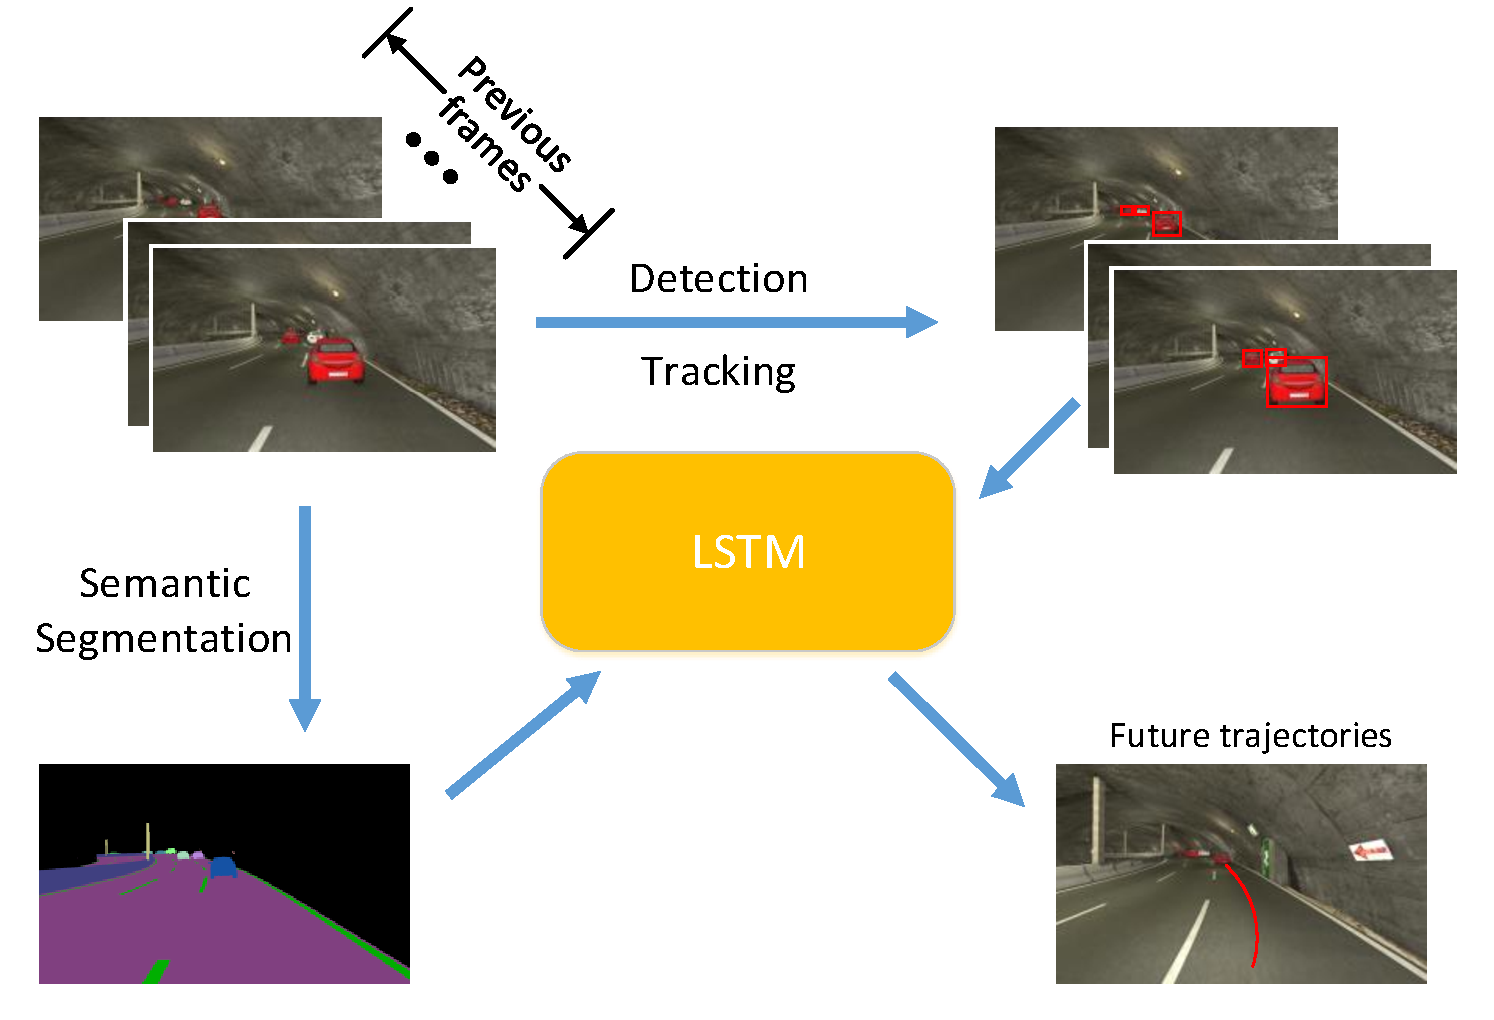
\includegraphics[width=0.45\textwidth]{figures/pull_figure.pdf}
        \caption{ {\small We propose a system to predict future trajectories of vehicles. Given a historical information, obtained by detection, tracking and semantic segmentation, a network based on Long Short Term Memory (LSTM) structure is trained to generate future information}}
        \label{fig:pull_figure}
\end{figure}

%\textbf{\emph{1.4. Why hasn't it been solved before? (Or, what's wrong with previous proposed solutions? How does mine differ?)}}
Vehicles trajectory prediction is also very related to visual tracking.
In traditional vision based tracking problems (\emph{e.g.},~\cite{wu2013online, wu2015object, mueller2016benchmark}) where target objects go through rather sporadic movements (usually the object trajectory is generated by artificial movement in order to test the robustness of the tracker), the prediction of target's future trajectory is simply a moot problem.
However, traffic participants generally exhibit regular trajectories (\emph{e.g.,} cars driving on the road, pedestrians walking on the sidewalks). Given law-abiding traffic participants, human drivers subconsciously project visual target's future trajectory.
Nonetheless, due to the missing bridge between traditional visual tracking community and current autonomous driving research community, there is a lack of proper metrics for evaluating the temporal prediction result.


%\textbf{\emph{1.5. What are the key components of my approach and results? Also include any specific limitations.}}

% Then have a final paragraph or subsection: "Summary of Contributions". It should list the major contributions in bullet form, mentioning in which sections they can be found. This material doubles as an outline of the rest of the paper, saving space and eliminating redundancy.
In our approach, there are three key components: traffic participants detection, instance tracking and future trajectory prediction as shown in Fig.~\ref{fig:pull_figure}.Our contributions are as follows:

\begin{itemize}

\item We verify the feasibility of predicting vehicles' future trajectories for assisting mediated perception. The proposed system stems from the issue of human driver reaction time in the autonomous driving context.

\item We present a novel ``tracking-by-detection" framework for robust vehicle tracking. By updating tracker's target representation via detection association, we also solve the problem of instance association between frames.

\item We design various temporal models for the problem of predicting future trajectories based on historical data. Results show that the temporal model generating intermediate representation performs better than the frame-to-frame based temporal model.

\item We demonstrate the effectiveness of using ``privileged information"(\emph{e.g.}, scene semantics) further boost the prediction accuracy.


\item We construct a time-series dataset for vehicle trajectory prediction based on the SYNTHIA dataset~\cite{ros2016synthia} and  formalize the problem into a 3D occupancy grid problem given depth information.

\end{itemize}



\section{Related Work}

%\textbf{\emph{1. Object detection, segmentation, instance segmentation}}
%\subsection{Traffic participants detection and tracking: object detection and instance association}
\subsection{Object detection}
Vehicle detection is one key component of an autonomous driving system. Typical algorithms output bounding boxes on detected vehicles.
A lot of progess has been made in recent years on object detection due to the use of convolutional neural networks (CNNs).
Modern object detectors based on these networks -- such as the line of works on the R-CNN~\cite{girshick2014rich},
Fast R-CNN~\cite{Girshick2015Fast}, Faster R-CNN~\cite{ren2015faster_nips}, Mask R-CNN~\cite{he2017mask} and  SSD~\cite{liu2016ssd} -- are now good enough to be deployed in a consumer products.
% Before the resurgence of convolutional neural network (CNN), Deformable Part Model (DPM) \cite{felzenszwalb2008discriminatively} and Selective Search \cite{Uijlings2013Selective} are the trend of this field.
% However, after the proposal of
 R-CNN~\cite{girshick2014rich} combines Selective Search and deep learning features to detect objects.
 % At the beginning, R-CNN is a step-by-step and inefficient method. Then,
  SPPNet \cite{He2015Spatial} exploits a spatial pyramid pooling layer to extract multi-scale deep features. Later Fast R-CNN~\cite{Girshick2015Fast} introduces the multi-task learning to fine-tune all layers in their network. At last, Faster R-CNN \cite{ren2015faster_nips} proposes a region proposal network (RPN) and integrates RPN and Fast R-CNN to build a end-to-end architecture. Meanwhile, SSD \cite{liu2016ssd} uses a series of boxes and directly gives the probability for each object class. In addition, YOLO \cite{redmon2016you} proposes a fast object detection method, which divides the input image into grids, then predicts object positions and confidences for each category in each grid.

%In the field of semantic segmentation, FCN~\cite{long2015fully} firstly transfers the fully-connected layers into convolution layers, turning the segmentation task into a pixel-wise classification task. Deeplab~\cite{chen2016deeplab} proposes a dilated convolution layer to explicitly control the resolution at
%which feature responses are computed within Deep Convolutional Neural Networks. DRN~\cite{yu2017dilated} further proposes a semantic network by integrating residual structure and dilated convolution.

%With the modification of neural network, conditional random field (CRF) is employed into refining the output of network in \cite{chen2016deeplab}. After that, CRF is merged into neural network to become an end-to-end architecture \cite{liu2015semantic,zheng2015conditional,arnab2016higher}


\subsection{Instance association}
Instance association between frames is a prerequisite to solve the proposed intrinsically temporal problems.  3D scene flow is estimated in~\cite{behl2017bounding} by exploiting recognition to overcome the challenging scenarios in the present of large displacement or local ambiguities.
%Their method achieve state-of-the-art performance on the KITTI2015 scene flow benchmark.
However, a total runtime of 10 minutes per frame is way too prohibitive for the deployment in the context of autonomous driving.
To accomplish the task of instance association between frames, we resort to the well studied field of visual tracking.
Discriminative Correlation Filters (DCF)~\cite{henriques2015high} have demonstrated excellent performance for high-speed generic visual object tracking.
Built upon their seminal work, there has been a plethora of recent improvements~\cite{wang2016stct, wang2015visual, hong2015online, ma2015hierarchical,danelljan2016beyond,held2016learning, wu2017kernalised,danelljan2017eco} relying on convolutional neural network (CNN) pretrained on ImageNet as a feature extractor for visual tracking.

\begin{figure*}[t]
        \centering
        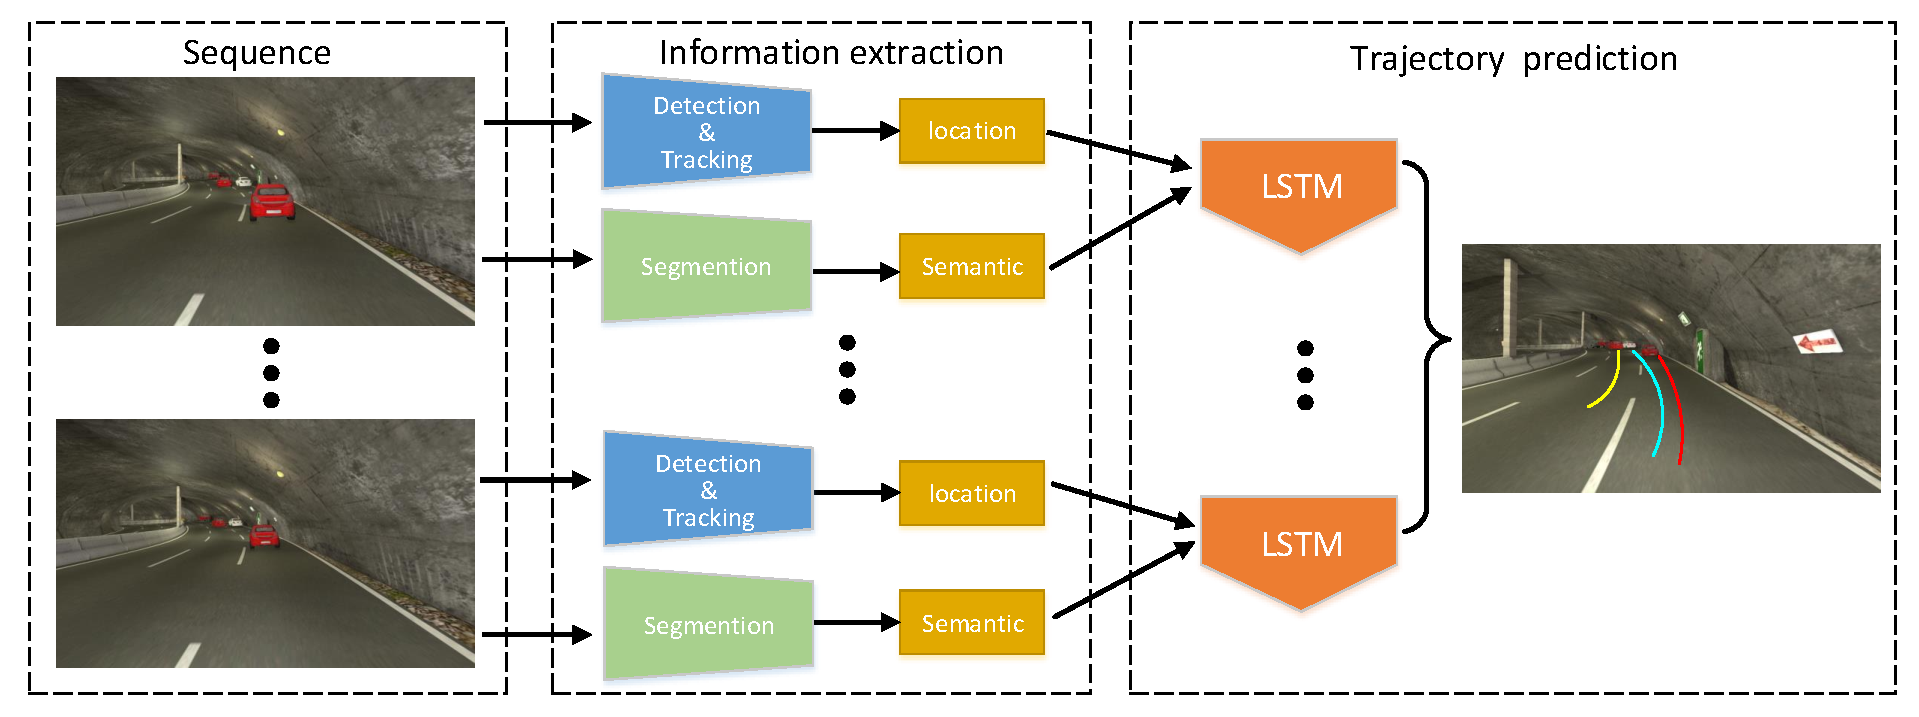
\includegraphics[width=0.75\textwidth]{figures/framework.pdf}
        \caption{ {\small The framework of our vehicle future trajectory prediction system. The input is the sequence data from a synthetic scene in \cite{mueller2016benchmark}. Historical information are extracted by detection & tracking and semantic segmentation. All of the information is fed into our LSTM model to predict future trajectories.}}
        \label{fig:framework}
\end{figure*}


\subsection{Recurrent neural networks}

Recent advances in recurrent neural network for modeling visual sequential data are also related to our work.
%Recently, RNN(recurrent network) and its variant LSTM(long short-term memory) have been successfully used in autonomous driving, due to its advantages for modeling sequential data in vision problems.
Mostly, RNN is trained as a pilot network in the context of behaviour reflex approaches.
Long Short Term Memory (LSTM) cells are usually exploited as one intermediate component of an end-to-end driving model.
 A combination of a fully-convolutional network and an LSTM is proposed in~\cite{xu2017end} to learn from large-scale vehicle action data. Their goal is to predict future egomotion including multi-modal discrete and continuous driving behaviors.
 Inverse turning radius is predicted by a LSTM network in~\cite{kim2017interpretable}: they generate a heat map of attention at each time step conditioned on the previous hidden states and a current convolutional feature cube  to produce more succinct visual explanations. ~\cite{duself} used 3D convolutional layers to extract visual features, then fed them into LSTM layers to capture the sequential relation. In addition to using deep features, ~\cite{koutnik2013evolving} trained a large recurrent neural network using a reinforcement learning approach to map images directly to steering angles, with the purpose to keep the car on track.



\subsection{Dataset for autonomous driving}

Vision-based semantic segmentation in urban scene is a key functionality for autonomous driving.
%Camvid dataset~\cite{Camvid} consists of a set of monocular images taken in Cambridge UK. However, only 701 images contain pixel-level annotations over a total of 32 categories (combining objects and architectural scenes).
%Similarly, Daimler Urban Segmentation dataset~\cite{scharwachter2013efficient} contains 500 fully labelled monochrome frames for 5 categories.
KITTI benchmark suite~\cite{Geiger2013IJRR} provides a large a mount of images of urban scene from Karlsruhe, Germany, with ground truth data for odometry, object detection, tracking, scene flow and stereo benchmarks. However, a limited 430 labelled images are provided for semantic segmentation.
%A common limitation of the aforementioned datasets is the bias introduced by the acquisition of images in a specific city. The LabelMe~\cite{russell2008labelme} project offers the solution by offering around 1,000 fully annotated images of urban environments around the world and more than 3,000 images with partial(noisy) annotations.
More recently, larger project are constructed:
Cityscapes dataset~\cite{Cordts2016Cityscapes} which consists of a collection of images acquired in 50 cities around Germany, Switzerland and France in difference seasons, and having 5,000 images with fine annotations and 20,000 with coarse annotations over a total of 30 classes. Comma.ai~\cite{santana2016learning} provides 7 and a quarter hours of largely highway driving. Udacity~\cite{udacity} dataset includes 65,000 labels across 9,423 frames at full resolution of $1920\times1200$ at 2Hz.
The use of synthetic data has increased considerably in recent years within computer vision community. A synthetic dataset named Synthia is\cite{mueller2016benchmark} provide originally for urban scene semantic segmentation generation.
%In~\cite{kaneva2011evaluation}, the authors used a photorealistic virtual world to evaluate the performance of image features under scene changes and image transformations. Synthetic data has also been used for skeleton joints estimation~\cite{shotton2013real}, allowing the classifier invariant to pose, body shape, clothing, etc.
Synthetic dataset has an obvious advantage: a fine annotated images in Cityscape dataset requires on average 1.5 hours which is very labor intensive. Thus, the cost of scaling large project would required a prohibitive economic investment in order to capture images from a larger variety of countries, in different seasons and different traffic conditions.
%For these reasons, a novel synthetic dataset of urban scene called SYNTHIA~\cite{ros2016synthia} is proposed to use synthetic imagery that simulate real urban scenes in a vast variety of conditions and produce the appropriate annotations.
%This dataset is a large collection of images with high variability due to changes in illumination, textures, pose of dynamic objects and camera view-points.

\section{Proposed Algorithm}

We first describe our overall approach for vehicle trajectory prediction and the details of implementation are presented in Sec~\ref{sec:Implementations}.
Our goal is via collecting the visual information from the past to predict the traffic participants future trajectory. Fig.~\ref{fig:framework} shows the overall architecture of our proposed framework.

\subsection{Generic 3D Traffic Participants Trajectory Prediction}

We propose to learn a generic approach from history information and formulate the problem as predicting future traffic participants' trajectories.
Our work is most related to~\cite{xu2017end} where the problem was to predict future feasible actions of egomotion from a motion reflex perspective.
We, instead,  predict other traffic participants' future trajectories.
Formally, our problem can be defined as a mapping between historical trajectory $ \{h_t^p\}, t=1,\dots, T $ with auxiliary information $ \{a_t^p\}, t=1,\dots, T $ for traffic participant $p$ and the future trajectory $\{j_t^p\}, t={T+1}, \ldots$:

\begin{equation}
\bm{\mathcal{M}}_p(h, a): H \times A  \rightarrow J
\label{eq:mapping}
\end{equation}
where the traffic participants $p$ can be of vehicles, cyclists, pedestrians, \emph{etc}. Historical and future trajectories are defined in a 3D occupancy grid:
\begin{equation}
H, J \in \Re^{6} =  \{x, y, w, h, d_{min}, d_{max}\}
\label{eq:mapping2}
\end{equation}
where $\{x,y,w,h\}$ define target's 2D boundingbox in image pixel space and $\{d_{min}, d_{max}\}$ define the minimum and maximum relative distance between host car and the tracking target acquired from the depth camera. Given RGB cameras' focal length $f$, the pixel space 2D boundingbox can be projected into 3D real-world coordinate $\{x_r,y_r,w_r,h_r\}$ as:
\begin{align}
    x_r = \frac{x}{f} \times d \\
    y_r = \frac{y}{f} \times d
\label{eq:focal_length}
\end{align}
where $d$ is distance between  the center of the lens and the center of target and we use $d_{min}$ as a close approximation.


Auxiliary information $A$ could be scene semantics to regularize the path of future trajectory or car pose information to decide whether it's an approaching car or a parallel driving car.


\begin{figure}[t]
        \centering
        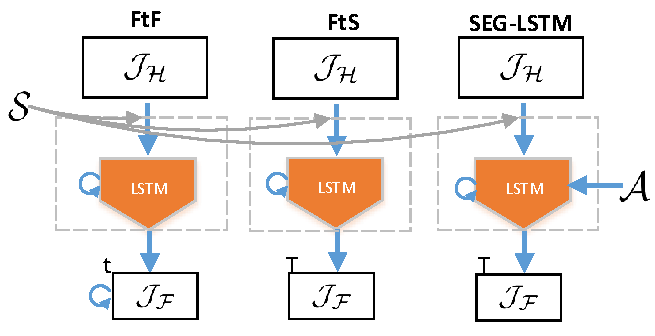
\includegraphics[width=0.5\textwidth]{figures/network_detail.pdf}
        \caption{ {\small Different networks to predict future trajectory. Left: FrameToFrame, .....; Middle:FrameToSeq, ....; Right:SEG-LSTM, ......}}
        \label{fig:dataset}
\end{figure}
\subsection{SEG-LSTM Architecture}


We compare two temporal models based on LSTM cells for predicting the car trajectory.
Results show that the temporal model generating intermediate output utilizing the whole historical data performs better than the frame-to-frame based output temporal model.





\subsection{focal lenes back projection into real world grid}



%%%%%%%%%%%%%%%%%%%%%%%%%%%%%%%%%%%%%%%%%%%%%%%%%%%%%%%%%%%%%%%%%%%%%%%%%%%%%%%%%%%%%%%%%%%%%%%%%%%%%%%%%%%
\section{Experiments}

\subsection{Dataset collection}

Currently, most public datasets with semantic labeling are single frame, static images. Continuous video streams are required for the purpose of car trajectory prediction.
We collect car trajectory prediction dataset based on the SYNTHIA~\cite{ros2016synthia} dataset.
SYNTHIA dataset is a large corpus of synthetic images originally collected for the purpose of semantic segmentation of urban scenes generated by rendering a virtual city created with the Unity development platform.
The potential of this virtual world includes extension capabilities: new parts of the cities and road conditions can be easily generated by adding different setups. The major features of the collected dataset include: scene diversity (European style town, modern city, highway and green areas), variety of dynamic objects (cars, pedestrians and cyclists), multiple seasons (dedicated themes for winter, fall, spring and summer), lighting conditions and weather (dynamic lights and shadows, several day-time modes, rain mode and night mode).
There are more than 200,000 HD ($760\times1280$) photo-realistic frames from video streams.
Frames are acquired from multiple view-points (up to eight views per location), and each of the frames also contains an associated depth map. In our experiment, we used only left front camera view data.

The focus of this paper is on car trajectory prediction on highways which corresponds to sequence number 1 in the SYNTHIA dataset. We especially concern about the cars that are relatively close to the driver.
In order to decide quantitatively which vehicles are close to the host car, we define pixel occupancy ratio \emph{(POR)} as the ratio between the total number of pixels of the tracking vehicle and the total number of pixels of the camera input.
As in accordance with~\cite{chen2015deepdriving}, we set the reliable car perception as 30 meters so as to guarantee satisfactory control quality when the speed of the host car does not exceed 72km/h.
Since depth information is also provided alongside in the SYNTHIA dataset, we back-projecting the segmented instance region onto the depth maps and estimate that the POR of 0.2\% and 0.1\% correspond to roughly 30 meters and 100 meters of relative distance between the host car and the tracking vehicle.
Hence, we start tracking the target when the POR of the detected vehicle is larger than 0.2\%  so as to suffice the safety distance for driver to make timely reaction and stop tracking the vehicle when the POR is smaller than 0.1\% indicating the target car is too far to influence driving policy.
We follow the prediction time allocation as in~\cite{xu2017end} that the historical time-span is 3 seconds (corresponds to 15 frames with 5 Hz frame rate in the SYNTHIA dataset).
However, in contrast with~\cite{xu2017end} where only the next 1/3rd of a second is predicted, we strive to predict the next 1.5 second's future trajectory as mentioned previously that it's the reaction time accident reconstruction specialists commonly used~\cite{mcgehee2000driver}.

We follow the traditional paradigm for visual tracking to collect target's bounding box: $[x, y, w, h]$ of each frame. Moreover, the minimum relative distance $d_{min}$ and maximum relative distance $d_{max}$ can also be acquired from the depth camera. The train/valid/test are split as 80\%/10\%/10\% of the total tracklets and the total numbers are shown in Tab.~\ref{tab:dataset_statistics}.
We list our logic for collecting continuous car tracking in List~\ref{list:dataset_collection}.
Some sample frames with semantic labels and depth information is shown in Fig.~\ref{fig:dataset}.

%%%%%%%%%%%%%%%%%%%%%%%%%%%%%%%%%%%%%%%%%%%%%%%%%%%%

\begin{algorithm}[h]
\begin{algorithmic}
\caption{\textbf{Car trajectory ground truth collection}}\label{list:dataset_collection}
\STATE \textbf{Step 1} $\rightarrow $ acquiring traffic participants from ground truth annotations with only ``car" as instances.
\STATE \textbf{Step 2} {$\rightarrow $ acquiring frame-based instance information:
{
\bindent
  \IF{POR $> 0.2\%$}
    %\bindent[1.45cm]
    \STATE $\Rightarrow$ start tracking instance;
    \STATE $\Rightarrow$ collecting 3D tracking boundingbox: $[x, y, w, h, d_{min}, d_{max}]$;
    \STATE $\Rightarrow$ collecting semantic labeling image $I_{seg}$;
    \STATE $\Rightarrow$ collecting 2D car pose from RGB input $I_{car}$;
    %\eindent
  \ELSIF{POR $< 0.1\%$}
    \STATE $\Rightarrow$ stop tracking.
    \ENDIF\eindent}
  }
\STATE \textbf{Step 3} $\rightarrow $ splitting sequences into tracklets of 23 frames with step size 1:
{\bindent
    \STATE $\Rightarrow$  first 15 frames (5Hz, 3 sec) as training input;
  \STATE $\Rightarrow$  next 8 frames (1.6 sec) as the held-up future trajectory to be predicted.
  \eindent}

\end{algorithmic}
\end{algorithm}
%%%%%%%%%%%%%%%%%%%%%%%%%%%%%%%%%%%%%%%%%%%%%%%%%%%%%%%%%%%%%%%%%%%%%%%%%%%%%%%%%%%%%%%%%%%%%%%%%%%%%%%%%%%%%%%%

\begin{figure}[t]
        \centering
        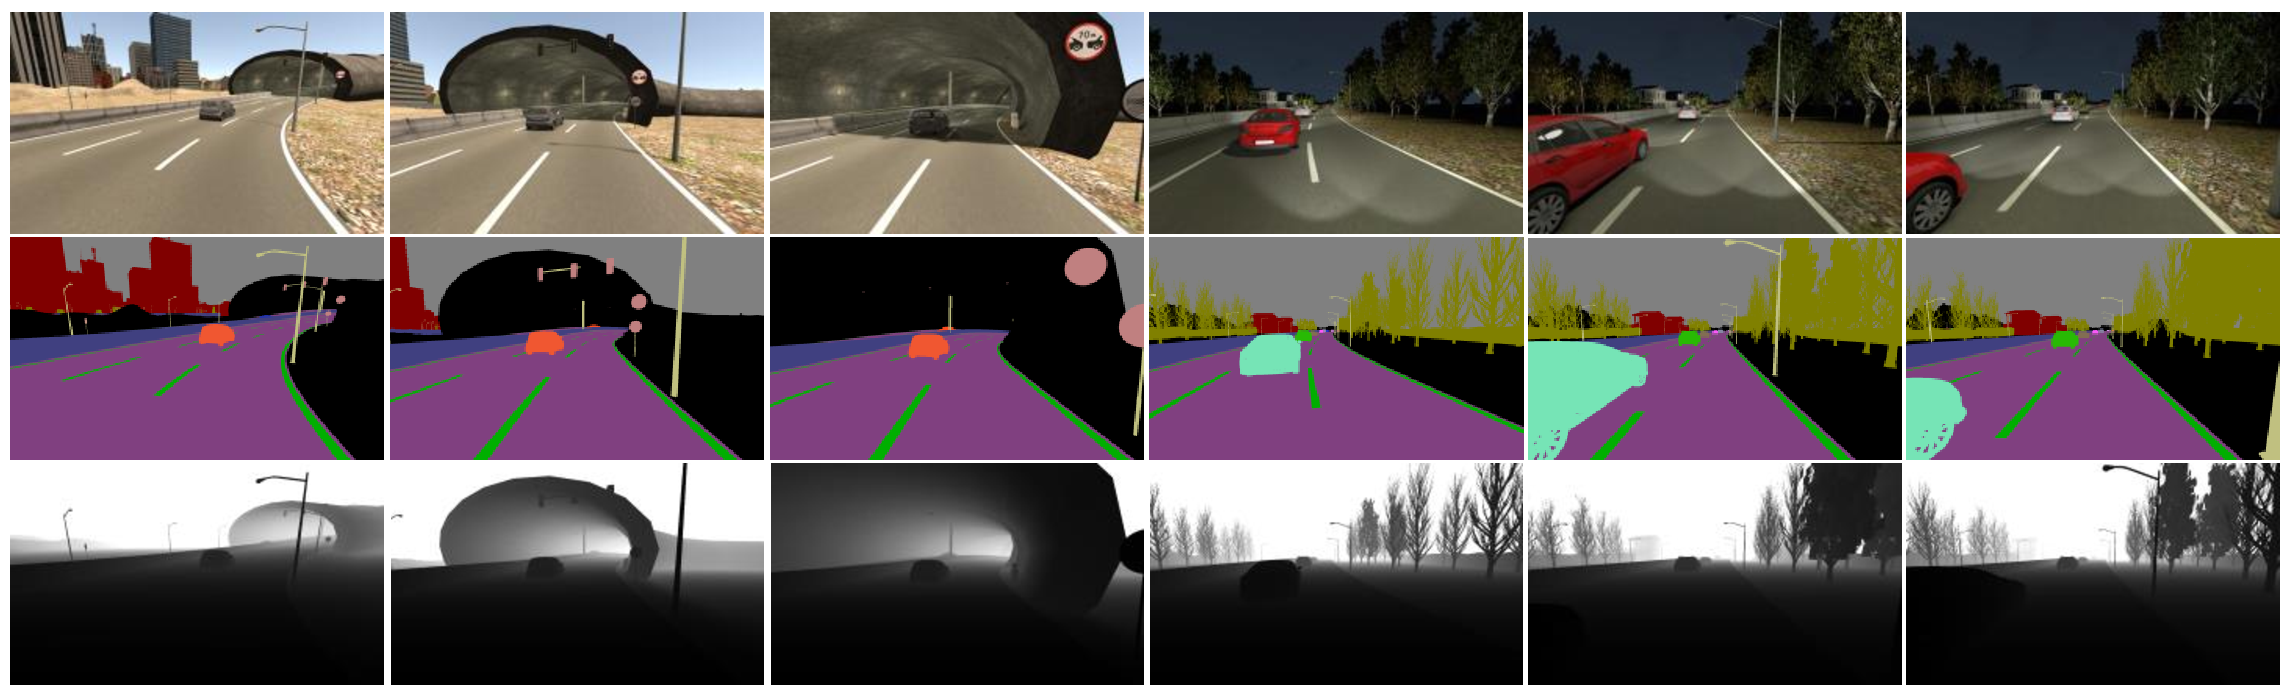
\includegraphics[width=0.5\textwidth]{figures/dataset.pdf}
        \caption{ {\small Examples of collected dataset for car trajectory prediction. From top to bottom: RGB, semantic labeling, depth maps for three continuous frames of two dynamic light conditions.}}
        \label{fig:dataset}
\end{figure}

%%%%%%%%%%%%%%%%%%%%%%%%%%%%%%%%%%%%%%%%%%%%%%%%%%%%%%%%%%%%%%%%%%%%%%%%%%%%%%%%%%%%%%%%%%%%%%%%%%%%%%%%%%%%%
%\begin{table}\centering
%\ra{1.}
%\begin{tabular}{@{}llll@{}}\toprule
%
%                & \#train & \#valid & \#test\\
% \hline
% tracklets      &  10400    &  1300    & 1280 \\
% \hline
% car detection  &   7832     & 976     & 986 \\
% \hline
% semantic segmentation  &  7841  & 977  & 987 \\
% \hline
%\end{tabular}
%\caption{Dataset statistics}
%\label{tab:dataset_statistics}
%\end{table}
\subsection{Implementations}\label{sec:Implementations}


\subsubsection{Traffic participants detection}

To reliably detect traffic participants, we compared two state-of-the-art approaches: SSD~\cite{liu2016ssd} and Faster-RCNN ~\cite{ren2015faster_nips}.
We use the pretrained network on the PASCAL VOC detection dataset~\cite{everingham2015pascal} which has 20 classes and fine-tune the network on the SYNTHIA with two classes: cars \emph{v.s.} background.
A comprehensive survey of trade-offs for modern convolutional object detectors is presented in~\cite{huang2017speed} and we refer keen readers to the aforementioned paper for a more complete comparison to achieve the right speed/memeory/accuracy balance for a given application and platform.

As it is also pointed out in the paper~\cite{huang2017speed} that SSD, albeit is less advantageous in detecting small object, it's very competitive for detecting larger objects. In this paper, we concerns mostly about cars that are close to the driver. Hence, given 0.1\% POR as the the cut-off threshold, the presented problem favors detectors that are robust in detecting larger objects.
Tab.~\ref{tab:ssd_fasterrcnn} also verifies that SSD is indeed more competitive when objects of interest are large in our problem set. We also compare the influence of confident score cut-off threshold and non-maximum suppression (NMS) threshold. It can been seen that both meta-architectures are robust to the cut-off confident scores.
In terms of the effect of NMS cut-off threshold, allowing larger threshold enables the detector to have slightly higher recall, it comes at a cost of multiple redundant overlapping detections and much lower f-score overall. In the following experiment, we adopt SSD with confident score of 0.5 as the cut-off threshold and 0.45 as the default jaccard overlap for NMS.


%\begin{table*}\centering
%\ra{1.}
%\begin{tabular}{@{}llllllllllll@{}}\toprule
%\multicolumn{2}{c}{conf}  & 0.5  & 0.55 & 0.6 &  0.65 & 0.7  & 0.75 & 0.8 &  0.85 & 0.9  & 0.95\\
%\hline
%\multirow{3}{*}{Faster-RCNN}
%                    &   precision & 81.2  & 81.2  & 81.1 & 81.1 & 81.1 & 81.0 & 81.0 & 80.7 & 80.5 & 80.0 \\
%                    &   recall    & 91.4  & 91.4  & 91.3 & 91.3 & 91.3 & 91.3 & 91.3 & 90.9 & 90.7 & 90.2\\
%                    &   f-score   & 86.0  & 86.0  & 86.0 & 86.0 & 86.0 & 86.0 & 86.0 & 85.5 & 85.3 & 84.8\\
%                    \cline{2-12}
%\multirow{3}{*}{SSD (NMS:0.60)}&   precision &  82.1  & 81.9  & 81.8  & 81.8  & 81.6  & 81.1 & 80.9  & 80.4 & 80.0  & 79.2\\
%                            &    recall   & \textbf{92.7} & 92.5 & 92.3  & 92.3 & 92.0 & 91.5 & 91.3 & 90.7  & 90.2 & 89.4\\
%                            &    f-score  & 87.1  & 86.9  & 86.7   &86.7&86.5& 86.0  & 85.8 &85.2 & 84.8 &84.0\\
%                    \cline{2-12}
%\multirow{3 }{*}{SSD (NMS:0.45)}&   precision & \textbf{92.0 } & 91.8 & 91.7 & 91.4 & 91.1 & 91.0 & 90.5 & 90.2 & 89.4 & 87.4\\
%                                &    recall  & 92.3  & 92.1 & 92.0 & 91.8 & 91.4 & 91.3 & 90.8 & 90.5 & 89.7 & 87.7\\
%                                &    f-score  & \textbf{92.2 } & 92.0 & 91.8 & 91.6 & 91.3 & 91.1 & 91.1 & 90.4 & 89.6 & 87.6\\
%
%\bottomrule
%\end{tabular}
%\caption{Caption: TODO results: (1) SSD better at detecting large object(which is in our case). (2) Faster-RCNN  is more robust to confidence threshold}
%\label{tab:ssd_fasterrcnn}
%\end{table*}

\subsubsection{Instance tracking}

The marriage between DCF~\cite{henriques2015high}, which has the advantage of being efficient in training translational images in the fourier space, and deep features, which excel at image representation, further advances the visual tracking community~\cite{qi2016hedged, danelljan2016eccv, wu2017kernalised, danelljan2017eco}. However, in the pursuit of ever increasing tracking accuracy, their characteristic speed and realtime capability have gradually faded. In the context of autonomous driving, accurate scale estimation of a target is also a prerequisite. Most state-of-the-art methods employ an exhaustive scale search to estimate the target size which is computationally expensive and struggles when encountering with large scale variations.
For this task, we adopt the real-time scale adaptive tracker fDSST~\cite{danelljan2017discriminative}.


\begin{figure}[t]
        \centering
        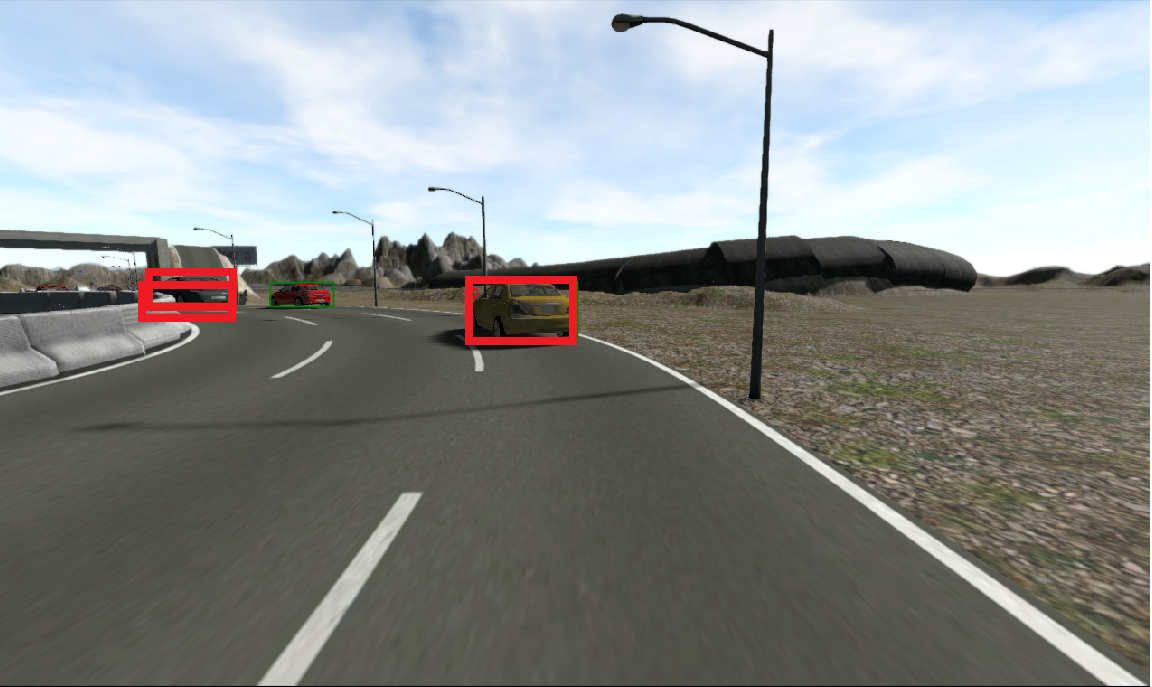
\includegraphics[width=0.4\textwidth]{figures/double_detection.png}
        \caption{ {\small TODO: Instance association caption goes here.}}
        \label{fig:Instance_associationn}
\end{figure}


\subsubsection{Semantic segmentation}
We use the state-of-the-art semantic segmentation networks: Dilated Residual Networks (DRN)~\cite{yu2017dilated}.

\subsubsection{Trajectory prediction}

We compare two temporal models based on LSTM cells for predicting the car trajectory.

TODO: compare the results using Kalman filtering.

%%%%%%%%%%%%%%%%%%%%%%%%%%%%%%%%%%%%%%%%


\subsection{Evaluation}
\begin{figure}[t]
        \centering
        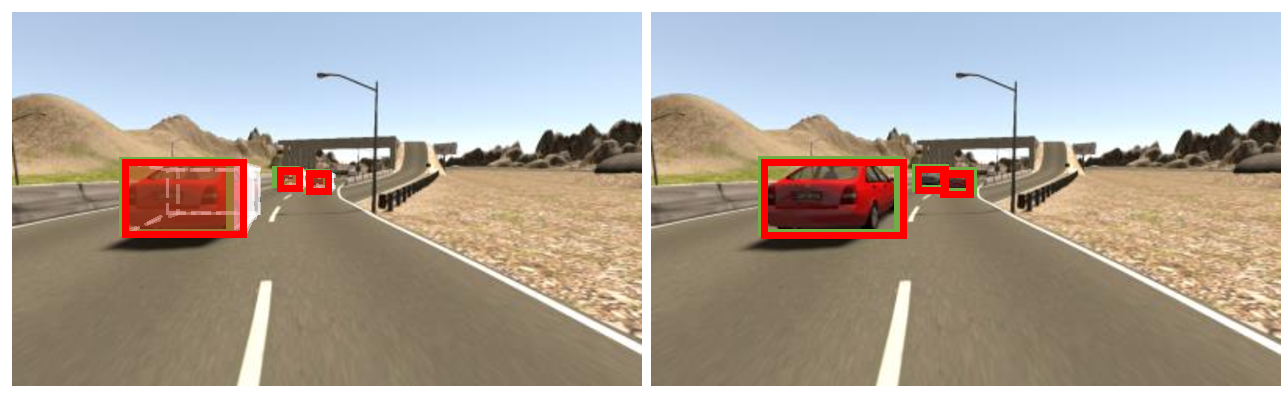
\includegraphics[width=0.5\textwidth]{figures/evaluation.pdf}
        \caption{ {\small TODO: The evaluation of 2D and 3D prediction. 2D: It is the bounding box to cover the whole vehicle. 3D: The depth channel is combined with 2D bounding box to predict trajectory.}}
        \label{fig:evaluation}
\end{figure}

%\begin{table}[t]
%\small
%   \centering
%        \begin{tabular}{|l|| *{2}{c}| *{2}{c} |}\hline
%            {\small Configuration} & \multicolumn{2}{|c|}{\small 2D}  & \multicolumn{2}{|c|}{\small 3D}  \\ \hline \hline
%                                                    & P20       & AUC       & P20       & AUC  \\ \hline \hline
%
%            {\small MTM }                          &  58.0     &  38.4     & 64.3      & 44.0   \\
%            \hline
%            {\small \textbf{MTFC} }  &  66.2 ${\color{red}(8.2\uparrow)}$    &  46.1 ${\color{red}(7.7\uparrow)}$    &  71.4 ${\color{red}(7.1\uparrow)}$     &  49.1 ${\color{red}(5.1\uparrow)}$\\
%            \hline
%            \hline
%            {\small MaxRes }                        &  57.5     &  38.8     &  65.8     &  45.9  \\
%            \hline
%            {\small \textbf{MTM (GT)} }        &  70.6${\color{red}(13.1\uparrow)}$     &  46.7  ${\color{red}(7.9\uparrow)}$   &  77.8 ${\color{red}(12.0\uparrow)}$    &  53.6 ${\color{red}(7.7\uparrow)}$ \\
%            \hline
%            \hline
%            {\small \textbf{MTFC}}           &  74.0${\color{red}(3.4\uparrow)}$      &  51.8${\color{red}(5.1\uparrow)}$      &  79.8${\color{red}(2.0\uparrow)}$      &  57.0${\color{red}(3.4\uparrow)}$    \\
%            \hline
%            {\small \textbf{DAC}}&  74.2 ${\color{red}(0.2\uparrow)}$    &  52.1${\color{red}(0.3\uparrow)}$     &  79.9${\color{red}(0.1\uparrow)}$     &  57.4${\color{red}(0.4\uparrow)}$\\\hline
%
%        \end{tabular}
%
%    \caption{ {\small
%         TODO: this table is just a place holder, currently has no meaning.}
%          } \label{table_baseline}
%\end{table}


%\begin{table}[t]
%\small
%   \centering
%        \begin{tabular}{|l|| *{2}{c}|}\hline
%            {\small Configuration} & \multicolumn{2}{|c|}{\small 2D}    \\ \hline \hline
%                                                  & P20       & AUC   \\ \hline \hline
%
%            {\small MTM }                          &  58.0     &  38.4      \\
%            \hline
%            {\small \textbf{MTFC} }  &  66.2 ${\color{red}(8.2\uparrow)}$    &  46.1 ${\color{red}(7.7\uparrow)}$  \\
%            \hline
%            \hline
%            {\small MaxRes }                        &  57.5     &  38.8   \\
%            \hline
%            {\small \textbf{MTM (GT)} }        &  70.6${\color{red}(13.1\uparrow)}$     &  46.7  ${\color{red}(7.9\uparrow)}$   \\
%            \hline
%            \hline
%            {\small \textbf{MTFC}}           &  74.0${\color{red}(3.4\uparrow)}$      &  51.8${\color{red}(5.1\uparrow)}$     \\
%            \hline
%            {\small \textbf{DAC}}&  74.2 ${\color{red}(0.2\uparrow)}$    &  52.1${\color{red}(0.3\uparrow)}$    \\\hline
%
%        \end{tabular}
%
%    \caption{ {\small
%    TODO: this table is just a place holder, currently has no meaning. WZN will update the numbers
%          Comparison with the most recent methods }
%          } \label{table_baseline2}
%\end{table}
%%%%%%%%%%%%%%%%%%%%%%%%%%%%%%%%%%%%%%%%%%%%%
\subsubsection{Evaluation Metrics}


\subsubsection{Baselines}
The Kalman filter is a popular technique for estimating the state of a system. Kalman filters estimate a continuous state and gives a uni-modal distribution. The Kalman filter represents all distributions of the Gaussians and iterates two things: (1) measurement updates; (2) motion updates


\begin{figure*}[t]
   \centering
    \begin{subfigure}[c]{0.4\textwidth}
    \centering
    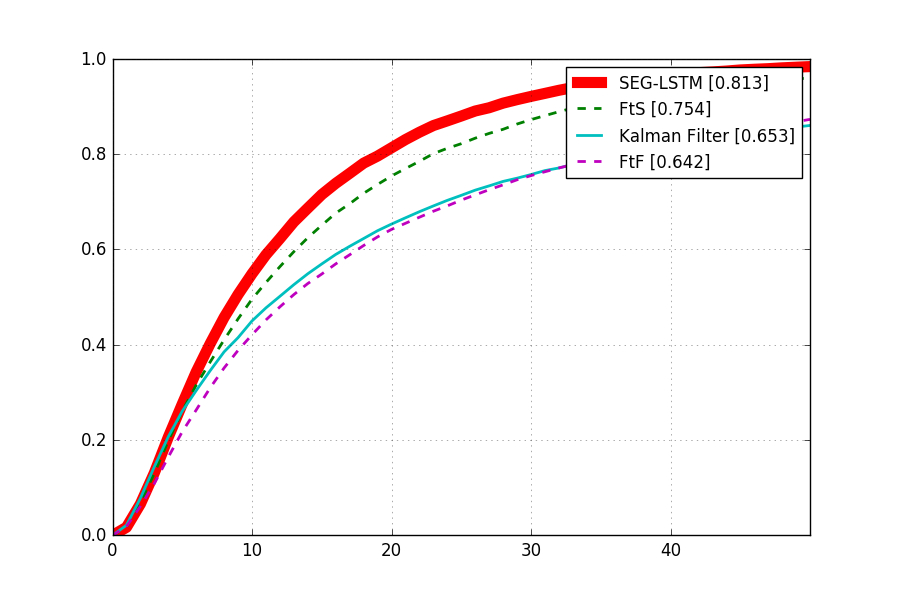
\includegraphics[width=7cm,height=5cm, clip]{figures/precision_plot_2d.png}
    \caption{\small{Precision plot for 2D}}
    \end{subfigure}%
    \begin{subfigure}[c]{0.4\textwidth}
    \centering
        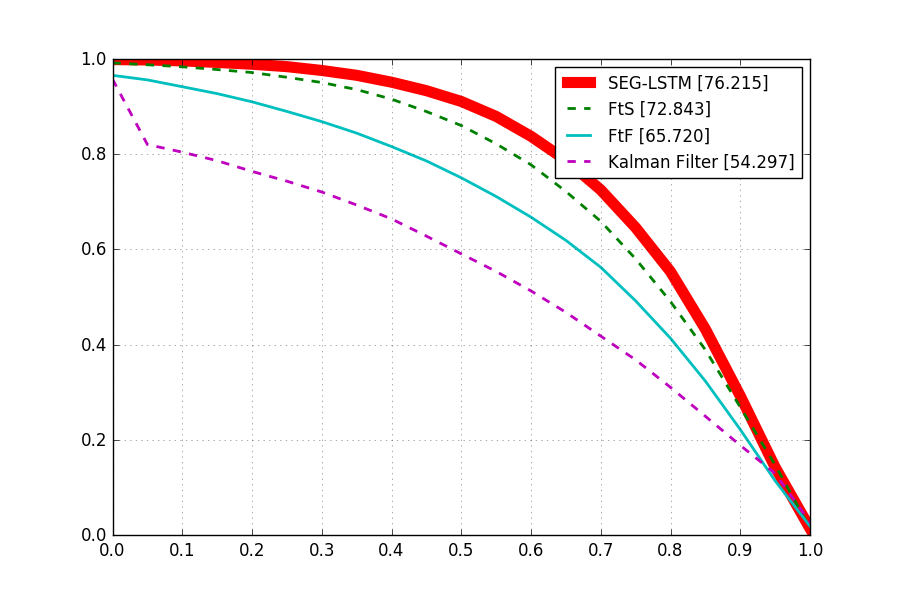
\includegraphics[width=7cm,height=5cm, clip]{figures/success_plot_2d.png}
        \caption{\small{Success plot 2D}}
    \end{subfigure}
    \\
     \begin{subfigure}[c]{0.4\textwidth}
     \includegraphics[width=7cm,height=5cm, clip]{figures/precision_plot_3d_20.png}
    \caption{\small{Precision plot for 3D}}
    \end{subfigure}%
    \begin{subfigure}[c]{0.4\textwidth}
    \centering
        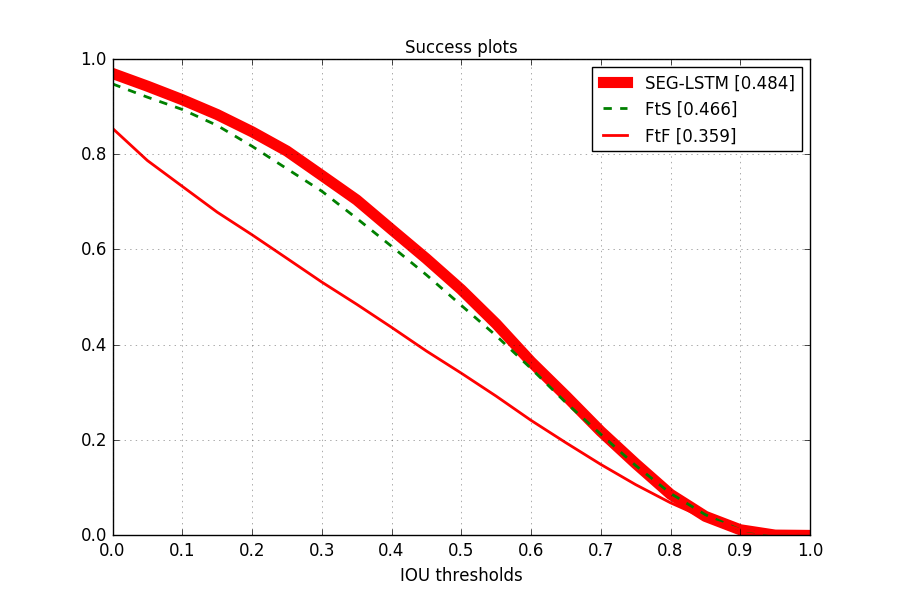
\includegraphics[width=7cm,height=5cm, clip]{figures/success_plot_3d.png}
        \caption{\small{Success plot 3D}}
    \end{subfigure}
\caption{Precision plot and success plot of the state-of-the-art, 2D, and 3D(TODO).
}
\label{fig:precision_plot_and_success_plot_OBT100}
\end{figure*}

\section{Conclusions}

Future works include incorporating vehicle pose from the RGB/depth input as extra source of ``privileged information"; conducting experiment on the real-world images.

\section*{Details of the Code}
 The code will be made public upon publication.

\section*{Acknowledgment}

{\small
\bibliographystyle{ieee}
\bibliography{egbib}
}
\end{document}
